%\documentclass[handout]{beamer} % normal aspect ratio
\documentclass[aspectratio=169]{beamer} % 16:9 aspect ratio (widescreen)

\usetheme{metropolis}           % Use metropolis theme

% load local layout definitions definitions
\newcommand*{\repositoryMainPath}{../../}%

\newcommand*{\templatePath}{\repositoryMainPath/template}%
\input{\templatePath/local_colors.tex} % colour definitions
\input{\templatePath/local_layout.tex} % footer, etc.

% shared folder
\newcommand*{\sharedPath}{\repositoryMainPath/shared}%


% import libraries
\usepackage[utf8]{inputenc}         %unicode support
\usepackage{adjustbox}
%\usepackage{algorithm2e}
\usepackage[ruled,vlined]{algorithm2e}
\usepackage{xargs}                      % Use more than one optional parameter in a new commands
\usepackage{bm}
\usepackage{colortbl}
%\usepackage[table]{xcolor}
\usepackage{csvsimple}
\usepackage{setspace}
\usepackage{tabularx}
\usepackage{amsmath}
\usepackage{amssymb}

\usepackage{etex}
\usepackage{tikz}
\usetikzlibrary{arrows,shapes,positioning}

\usetikzlibrary{arrows.meta}
\usetikzlibrary{trees}
\usetikzlibrary{graphs}
\usetikzlibrary{calc}
\usetikzlibrary{fit,positioning}
\usetikzlibrary{matrix}
\usetikzlibrary{shapes.symbols,patterns}

\usepackage{amsmath}
\usepackage{amssymb}
\usepackage{listings}
\usepackage{booktabs}
\usepackage{pdfpages}
\usepackage{mathtools}
\usepackage{enumerate}
\usepackage{multirow,tabularx}
\usepackage{booktabs}
\usepackage{pdfpages}
\usepackage{proof}
\usepackage{cancel}
\usepackage{chronology}
\usepackage{graphicx}
\usepackage{ulem}
\usepackage{amsmath}
\usepackage{amssymb}


\DeclareMathOperator*{\argmax}{arg\ max}
\DeclareMathOperator*{\argmin}{arg\ min}
% \DeclareMathOperator*{\min}{min}

\usepackage{mathrsfs}



\usepackage{xfrac}
\usepackage{nicefrac}

\usepackage{pgfplots}
\pgfplotsset{compat=1.12}

%\usefonttheme{professionalfonts} % using non standard fonts for beamer
%\usepackage{fontspec}
%\usefonttheme{serif}
%\setmainfont{Helvetica Neue}

\newcommand{\drawaline}[4]{
\draw [extended line=1cm,stealth-stealth] (#1,#2)--(#3,#4);
}
\usepackage{array}

\newcolumntype{L}[1]{>{\raggedright\arraybackslash}m{#1}}
\newcolumntype{C}[1]{>{\centering\arraybackslash}m{#1}}
\newcolumntype{R}[1]{>{\raggedleft\arraybackslash}m{#1}}


%\usepackage{enumitem}
%\setlist{nolistsep}



%%%%%%%%
% tikz defs

\input{\sharedPath/tikzSets}


% additional stuff

\newcommand{\etal}{{\em et al. }}
\newcommand{\markit}[1]{{\color{mydarkblue}{\bfseries#1}}}
\newcommand{\mathmarkit}[1]{\text{\color{mydarkblue}{$#1$}}}
\newcommand{\myBox}[2]{\begin{center}\begin{minipage}{#1\textwidth} #2 \end{minipage}\end{center}}


\title{M3.L3: Semantics and Ontologies}
\date{27.11.2019}
\author{Luke Slater (l.slater.1@bham.ac.uk)}
\institute{University of Birmingham - CCB - MSc Bioinformatics - Module 3}

% Either take the title from the docoment or define yourself - \thepresentationtitle is used in the footer
% V1: Take from presentation
%\def\title#1{\gdef\@title{#1}\gdef\thepresentationtitle{#1}}
% V2: Define yourself
\def\thepresentationtitle{MSc Bioinformatics - Module 3 - Lecture: 3: Semantics \& Ontologies}

\begin{document}

\small
\setlength{\abovedisplayskip}{4pt}
\setlength{\belowdisplayskip}{4pt}

\maketitle

\section{Introduction}

\begin{frame}{Objectives}
\begin{itemize}
  \item Just Semantics
  \item How do we express and represent knowledge?
  \item How can computers express and represent knowledge?
  \begin{itemize} 
    \item HTML: a degenerate form of XML
    \item XML: a degenerate form of RDF
    \item The Resource Description Framework (RDF)
  \end{itemize}
  \item Ontologies
  \begin{itemize} 
    \item What are they?
    \item What do they know? Do they know things? Let's find out!
    \item Differences between ontologies \& databases
    \item Ontologies in the real world
  \end{itemize}
  \item Afternoon: Practical
\end{itemize}
\end{frame}

\section{Knowledge Representation}

\begin{frame}{Moving from Information to Knowledge and Wisdom}
\begin{columns}
\column{0.5\textwidth}

\centering{
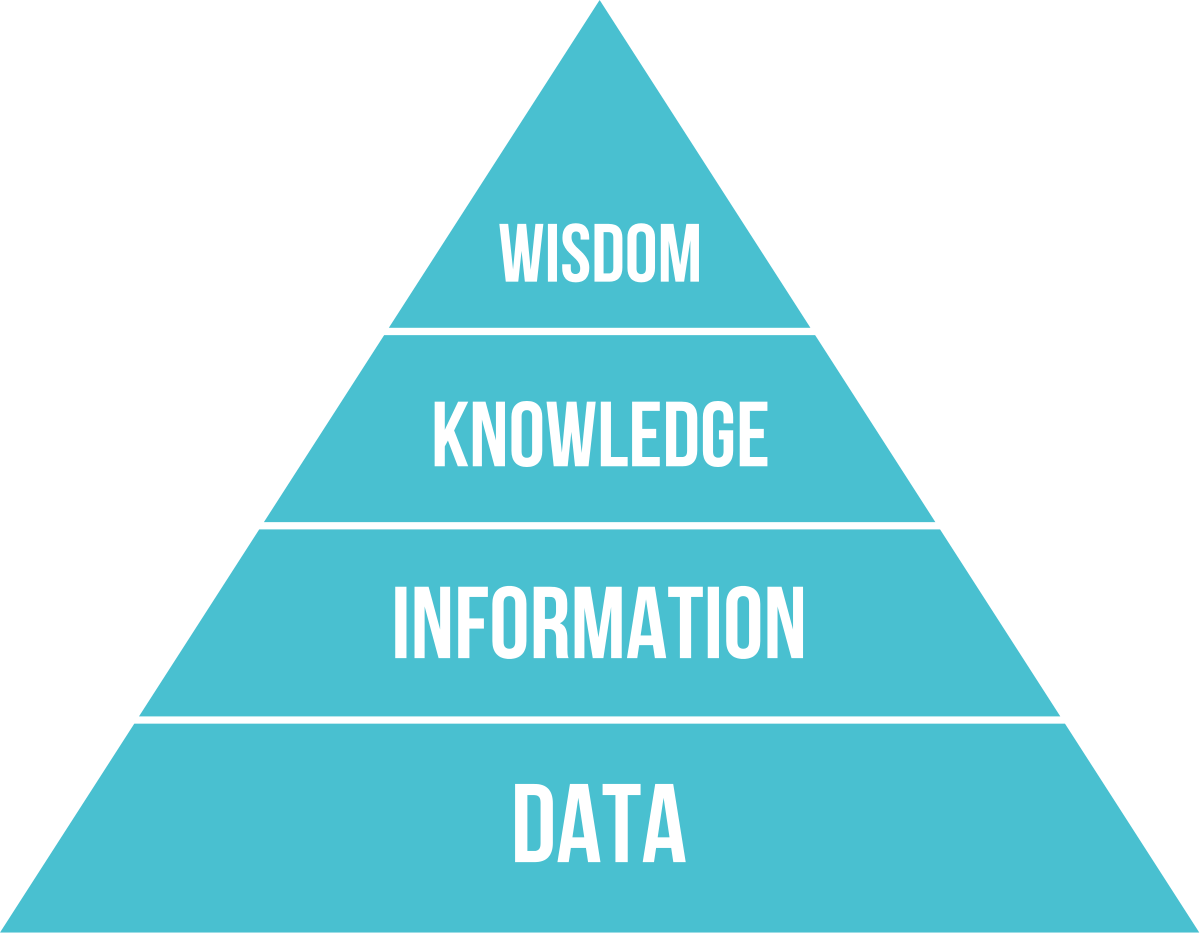
\includegraphics[width=\textwidth]{resources/pyramid.png}
}

\column{0.5\textwidth}

\begin{itemize}
  \item In learning databases, you will have learned how to take some data and store it as information on a computer.
  \item You have also learned how to create programs that use that data as knowledge.
  \item Now we will question what it is exactly that makes that data mean anything.
  \item We will also consider what it takes for a computer to have knowledge, and how we can move from knowledge to wisdom.
\end{itemize}

\end{columns}

\end{frame}

\begin{frame}{Epistemology}
  \begin{itemize}
    \item What does it mean to know something? What is knowledge? Even for humans, it is an unsolved
    problem.
    \item For a long time, Justified True Belief was regarded as an adequate
    solution for the question of what it means to know something. You can be said
    to know something if your assertion meets the following conditions:
    \begin{enumerate}
      \item You \emph{believe} the proposition is true.
      \item Your belief is somehow \emph{justified} (you have a reason to believe
      it).
      \item The proposition itself is \emph{true}.
    \end{enumerate}
    \item In 1963, Edmund Gettier released a mere 3-page paper defeating this notion by
    introducing the Gettier Problem\ldots
    \item Nevertheless, we persist with this general idea of knowledge, for the
    most part.
  \end{itemize}
\end{frame}

\begin{frame}{Wisdom Definition}
\large{Likely as many definitions as there are people who know the word, but in
this case we mean: the ability to think and act using \emph{knowledge}.}

\end{frame}

\begin{frame}
\frametitle{Symbols: Treachery of Images}

\centering{

\includegraphics[width=0.60\textwidth]{resources/pipe.jpg}
}
\end{frame}

\begin{frame}
\frametitle{Symbols and their Meanings}

\begin{itemize}
  \item This treachery lies not only in what might be called a picture, but also
  in words. For words are just another kind of image, or symbol.
  \item And so, what does it actually mean to be that which we refer when we say
  \emph{pipe}?
  \item And how does the symbol \emph{pipe} come to carry this meaning?
  \item Do these language symbols somehow
  directly correspond to reality (as in a picture), or are they very human mental
  constructs pointing vaguely at reality? (former: see Wittgenstein, latter: see
  later Wittgenstein).
\end{itemize}
\end{frame}

\begin{frame}
\frametitle{Consensus Meaning}

\begin{itemize}
  \item These symbols are imbued with meaning by a complex cultural process of
  consensus, which is in a state of constant flux and ambiguity.
  \item We further describe both particular objects (you) and classes of objects
  (Human) with complicated syntactic forms, from which meaning is also derived
  in a cognitive process fraught with constant flux and ambiguity.
  \item Things are complicated further when we consider what might be said 
  about an abstract noun, such as peace, green, or disco.
\end{itemize}
\end{frame}

\begin{frame}
\frametitle{The Syntactic Web}
\begin{itemize}
  \item We all know the syntactic web: the sum of human knowledge presented in natural 
  language, and intended for human interaction.
  \item As such, meaning is derived and agreed by offline consensus.
  \item Examples: Wikipedia, BBC news, Facebook, most websites as you know them.
  \item But how do we make computers understand it? Can computers understand it?
\end{itemize}
\end{frame}

\begin{frame}
\frametitle{Computers:}

\begin{itemize}
  \item Can count higher than you
  \item Needs to be a supercomputer to identify a dog
\end{itemize}
\centering{
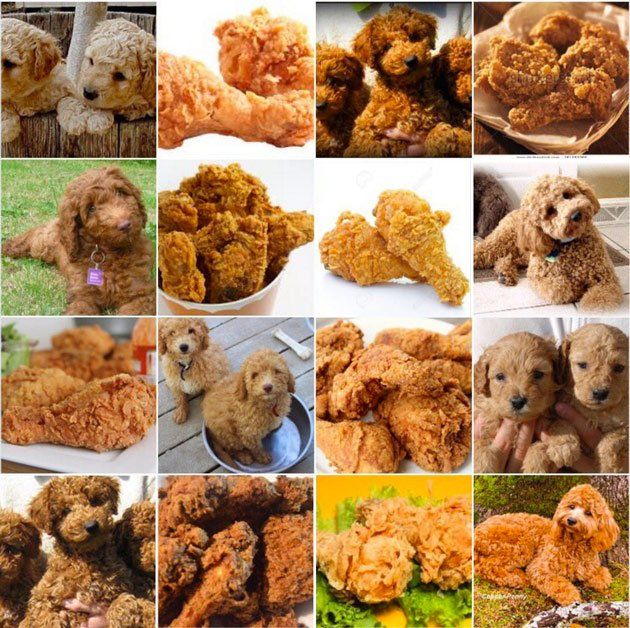
\includegraphics[width=0.4\textwidth]{resources/dog.jpg}
}
\end{frame}

\begin{frame}
  \begin{itemize}
    \item But for written language, why can't we solve all our problems with natural language processing?
    \item Indeed, we can `parse' natural language with computers\ldots
  \end{itemize}
\end{frame}

\begin{frame}
\frametitle{Natural Language Processing}

\centering{
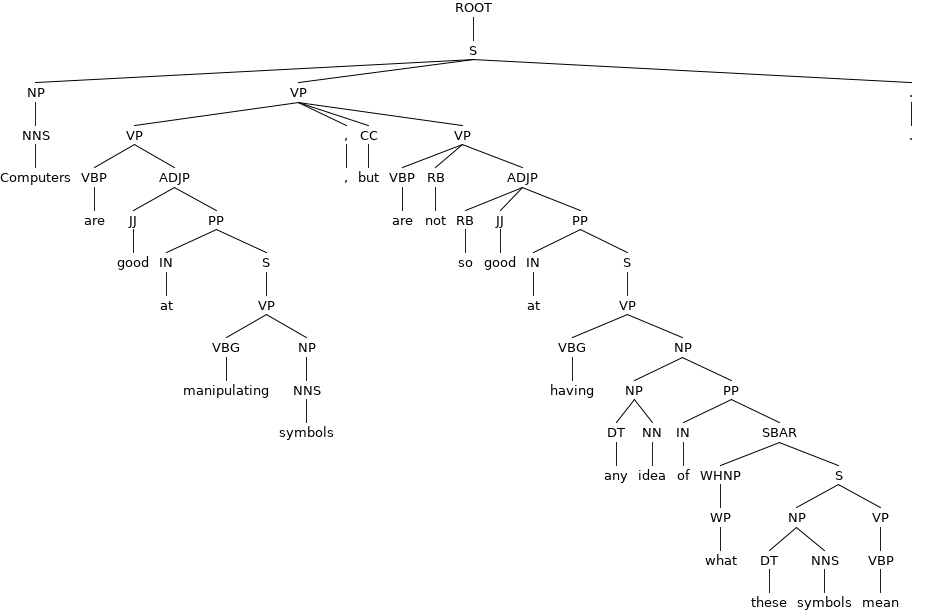
\includegraphics[width=0.8\textwidth]{resources/nlp.png}
}
\end{frame}

\begin{frame}
\frametitle{Limitations of Classical Natural Language Processing}

\begin{itemize}
\item Consider the sentence "I made her fish," which has at least five potential
meanings (double for plurality!):

\begin{enumerate}
  \item I cooked a fish for her.
  \item I cooked a fish belonging to her.
  \item I created the fish she owns.
  \item I forced her to go fishing.
  \item I made her into the Platonic ideal Fish.
\end{enumerate}

\item All problems in NLP may be reduced to the question of ambiguity - and it is
\emph{everywhere}; in human language, symbolic equivalence is not equivalent to semantic equivalence.
\item Even without the problem of ambiguity, who's to say what any of these words mean?

\end{itemize}
\begin{minipage}[t][.2\textheight]{\textwidth}
\tiny{Example inspired by "Speech and Natural Language
Processing" 2nd ed by Daniel
Jurafsky \& James H. Martin.}
\vfill
\end{minipage}
\end{frame}

\begin{frame}
\frametitle{The Limitation: Ambiguity and Meaning}

\begin{itemize}
  \item Computers are good at manipulating symbols, but are not so good at
  having any idea of what these symbols mean - their semantics.
  \item Furthermore, they struggle to translate symbols from ambiguous (read:
  human) languages into definite symbols to manipulate.
\end{itemize}
\end{frame}

\begin{frame}
\frametitle{The Problem}

\begin{itemize}
  \item How do we make a computer \emph{understand} the objects that we're describing,
  and the relationships between them?
  \item How can we make a computer \emph{know} something?
  \item How can we gain wisdom from the knowledge we give a computer?
  \item Requirements:
  \begin{enumerate}
    \item To be able to describe and to predicate upon \emph{particular}
    entities. For example: \emph{this gibbon is very angry}, or \emph{this tomato is
    mouldy}.
    \item To be able to define the \emph{kinds of} entities which may exist, and
    the relationships they may have between them. For example: \emph{a hand may have
    fingers}, or \emph{a parent must have a child}.
  \end{enumerate}
\end{itemize}
\end{frame}

\begin{frame}
\frametitle{Separating the entity and the instance}
 \begin{itemize}
  \item This separation of the class and the particular is along the lines of
  the Plato's Theory of Forms, or more generally Idealism: that particular
  objects (a chair) are partaking in a pure form which idealises and represents
  the most accurate reality of that object (The Chair or Chairness).
  \item This is one solution to the metaphysical problem of Universals.
  \item While rife with philosophical problems (much like any alternative
  theory), it happens to be extremely useful to us: computer scientists may
  notice a strong correlate when considering Object Orientated Programming:
  Classes and Instances.
\end{itemize}
\end{frame}

\begin{frame}
\frametitle{The Semantic Web}

\begin{itemize}
  \item Utilises the infrastructure of the world wide web as a data
  communication methodology.
  \item Instead of only presenting data: link, interpret, and analyse data.
  \item In the consumer sphere this forms the basis for the 'Internet of
  Things.' 
  \item Define things semantically in terms of how they relate to other things - their context.
\end{itemize}
\end{frame}

\begin{frame}
\frametitle{Describing instances}

\begin{columns}
\column{0.5\textwidth}


\includegraphics[width=\textwidth]{resources/html.jpg}

\column{0.5\textwidth}

Almost accidentally, the means by which we could develop a semantic
framework for knowledge representation was already in heavy use throughout the
world wide web.

\end{columns}
\end{frame}

\begin{frame}
\frametitle{HTML}
Web pages are created in HyperText Markup Language (HTML)
\begin{columns}

\column{0.6\textwidth}

\begin{lstlisting}[language=HTML]
  <p>Patient x has these symptoms:</p>

  <ul>
    <li>Hypertension</li>
    <li>Heart disease</li>
    <li>Right ventricular hypertrophy</li>
  </ul>
\end{lstlisting}

\column{0.4\textwidth}

Patient x has these symptoms:

\begin{itemize}
  \item Hypertension
  \item Heart disease
  \item Right ventricular hypertrophy
\end{itemize}

\end{columns}
\end{frame}

\begin{frame}
\frametitle{Natural Language Inference}

\begin{itemize}

\item As humans reading the list, he assertions we can infer from this text are numerous:

\begin{enumerate}
  \item A person exists.
  \item A person is a patient.
  \item There is at least one person.
  \item There is at least one patient.
  \item The patient has something wrong with their heart.
  \item At least one person has hypertension, heart disease, right ventricular hypertrophy.
  \item One person can have hypertension, heart disease, right ventricular hypertrophy simultaneously.
  \item \ldots
\end{enumerate}

\end{itemize}

\end{frame}

\begin{frame}
\frametitle{HTML: A Degenerate Form of XML}

\begin{itemize}
  \item HTML was later generalised, to create the eXtensible Markup Language
  (XML), without a focus on describing how a document should be rendered
  visually.
  \item This is a more general markup language, which can organise and "mark up" 
  or extend any kind of textual data with any additional information.
\end{itemize}

\end{frame}

\begin{frame}
\frametitle{RDF: An Exhilirate Form of XML}

\begin{itemize}
  \item A method of representing structured data for the semantic web.
  \item Used heavily within science for experimental results, datasets and
  various open data, particularly in the biological and biomedical domains.
\end{itemize}

\centering{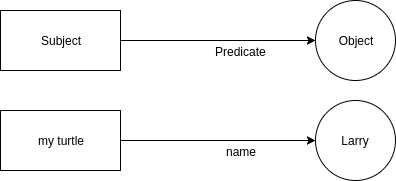
\includegraphics[width=0.7\textwidth]{resources/two.png}}
\end{frame}

\begin{frame}
\frametitle{RDF: Semantic Networks}
\centering{
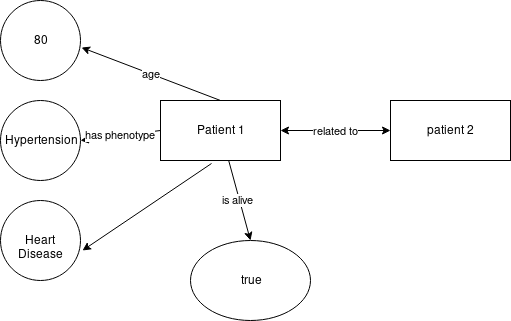
\includegraphics[width=0.7\textwidth]{resources/bands.png}
}
\end{frame}

\begin{frame}
\frametitle{Wikipedia vs DBPedia (syntactic vs semantic web)}
\begin{columns}

\column{0.5\textwidth}

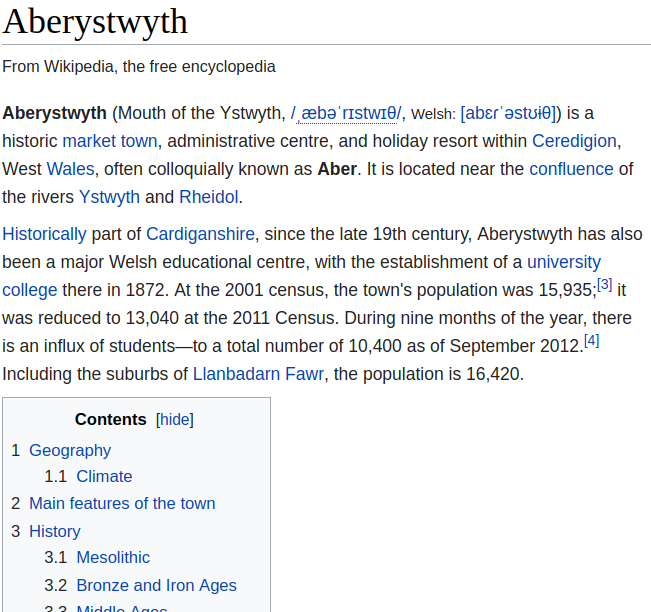
\includegraphics[width=\textwidth]{resources/aberwiki.png}

\column{0.5\textwidth}

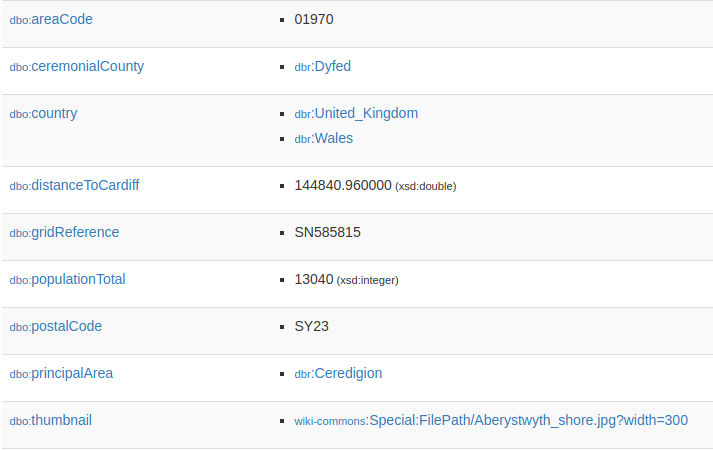
\includegraphics[width=\textwidth]{resources/aberpedia.png}

\end{columns}
\end{frame}

\section{Ontologies}

\begin{frame}
\frametitle{What is an ontology, anyway?}

\centering{

\includegraphics[width=0.5\textwidth]{resources/questionowl.png}
}

\end{frame}

\begin{frame}
\frametitle{Ontology: Describing Kinds of Objects} \begin{itemize}
  \item Ontologies categorise, define and relate the kinds of things in a domain.
  \item Easily thought of as the 'schema' for the data represented by RDF (and
  in any other format).
  \item For example, we've talked about patients and diseases - but how do we define patients and diseases themselves?
  \item Exact definitions differ, but most ontologies share four main features:
  \begin{enumerate}
    \item Classes and relations.
    \item Domain vocabulary.
    \item Metadata and descriptions.
    \item Axioms and formal definitions.
  \end{enumerate}
\end{itemize}
\end{frame}

\begin{frame}
\frametitle{Ontology: Classes (and relations)}
\begin{itemize}
  \item A class is a category of things which can exist within a
  particular world, defined by the necessary and sufficient conditions for a
  thing to exist within that category (intensional definition).
  \item Each distinct class has its own IRI (Internationalised Resource
  Identifier), but may share labels, descriptions, or any other information with
  other classes.
  \item This does not necessarily make them semantically equivalent!
  \item e.g. HP:0002457 and MP:0000436 both have the label 'abnormal head
  movements'
\end{itemize}
\end{frame}

\begin{frame}
\frametitle{Ontology: (Classes and) relations}
\begin{itemize}
  \item Also concerned with the relationships between things. A fundamental
  relationship between classes is the is-a relationship.
  \item All ontologies start with the root class \emph{Thing}, and all other 
  classes in the ontology stand in a transitive subclass relationship to it.
  \item In this way, they form, at a most basic level, a taxonomy of
  categorisation for a particular universe of interest.
  \item Other common relationships are: part-of, inheres-in, caused-by,
  regulates.
  \item Many relationships carry deeply argued issues and side-effects: fingers!
\end{itemize}
\end{frame}

\begin{frame}
\frametitle{Ontology: Domain Vocabulary}

\begin{itemize}
  \item Structured vocabulary for a domain
  \item Usually provided in the form of short 'labels' for each class (can have
  multiple)
  \item Provision for translated terms for classes
  \item Synonyms; the same category of things in a different context
  \item Together with the structure of the ontology, we gain a large and
  well-organised set of relevant terms for our domain
  \item Reduces ambiguity and misunderstanding in the conceptualisation for a
  domain
\end{itemize}
\end{frame}

\begin{frame}
\frametitle{Ontology: Domain Vocabulary}
\centering{
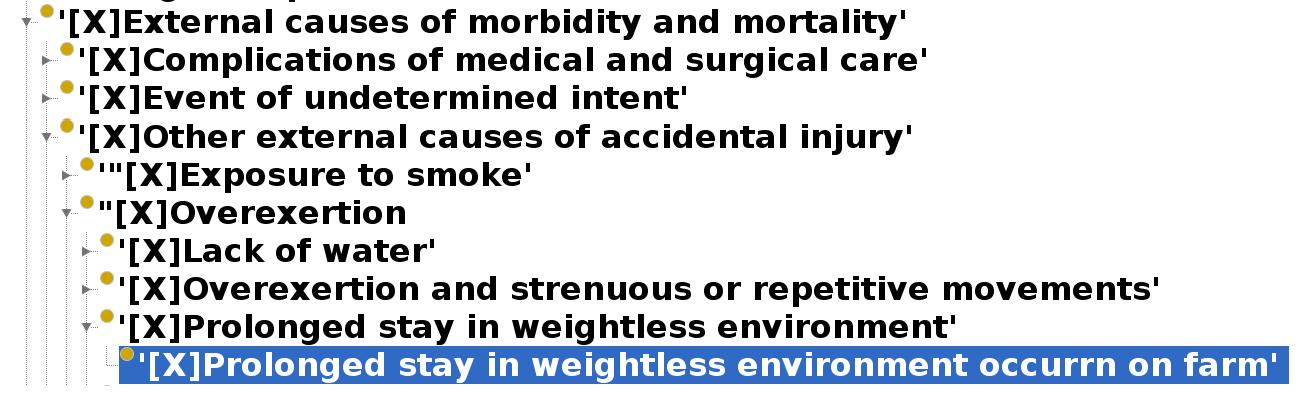
\includegraphics[width=\textwidth]{resources/read.jpg}
}
\end{frame}

\begin{frame}
\frametitle{Ontology: Metadata and Descriptions}

\begin{itemize}
  \item Descriptions, usually provided using the genus-differentia method.
  \begin{description}
    \item[temporal pattern] The speed at which disease
    manifestations appear and develop.
    \item[insidious onset] \textcolor{red}{Gradual, very slow}
    \textcolor{blue}{onset of disease manifestations}
  \end{description}
  \item Database cross-links, providing an assurance of semantic equivalence to
  data about an entity from an external source.
  \item Synonyms, broad or narrow
\end{itemize}
\end{frame}

\begin{frame}
\frametitle{Ontology: Axioms and Formal Definitions}

\begin{itemize}
  \item The formal aspect of ontologies, axiomatic expression of meaning.
  \item Example: hypertension defined as \textcolor{green}{has part}
  \textcolor{red}{some} ((\textcolor{blue}{blood} \textcolor{red}{and}
  (\textcolor{green}{part-of} \textcolor{red}{some} \textcolor{blue}{arterial
  system})) \textcolor{red}{and} (\textcolor{green}{has-quality}
  \textcolor{red}{some}
  ((\textcolor{blue}{increased pressure} \textcolor{red}{and}
  (\textcolor{green}{has-modifier} \textcolor{red}{some}
  \textcolor{blue}{chronic})) and (\textcolor{green}{has-modifier}
  \textcolor{red}{some}
  \textcolor{blue}{abnormal}))))
  \item Enable semantic analysis and (ostensibly) cross-species integration of
  knowledge.
  \item In many common ontologies phenotype axioms use the EQ (Entity-Quality) pattern
  \item We can also use these statements to query ontologies!
\end{itemize}
\end{frame}

\begin{frame}
\frametitle{Ontology Reasoning}

\begin{itemize}
  \item Reasoning is the use of a classifier to evaluate all logical consequences
  of the explicit statements in an ontology.
  \item This allows us to infer new knowledge, and evaluate the consistency of our
  logical model (and can tell us why in the case of inconsistency).
  \item There are many different reasoners, which use slightly different methods
  and support different subsets of description logic (they are often said to have
  different levels of ‘expressivity’).
\end{itemize}
\end{frame}

\begin{frame}
\frametitle{How do ontologies differ from databases?}

 \begin{table}[ht]
    \centering
    \begin{tabular}{|l|l|}
      \hline
      Database & OWL Ontology \\
      \hline
      Closed World Assumption & Open World Assumption \\
      Unique Name Assumption & No UNA \\
      Schema constraints data structure %, defining legal states of
                                %the database 
               & Axioms behave like inference rules\\\hline
    \end{tabular}
\end{table}
\end{frame}

\begin{frame}
\frametitle{Web Ontology Language (OWL)}

\begin{itemize}
  \item Reference to Winnie the Pooh.
  \item Based on description logics, a fragment of first order logic.
  \item A set of language specifications based on description logics.
  \begin{description}
    \item[Full] Every construct in OWL is available. Fully undecidable to
    reason. Cardinality restrictions, domain, range, and value restraints.
    \item[EL] Subset of OWL which is guaranteed to be classifiable in polynomial
    time. Only way to reach inconsistency is through disjointness.
    \item[RL] A subset which mirrors the features of relational databases.
  \end{description}
  \item Less expressive reasoners can simply ignore the more expressive content
  within ontologies.
\end{itemize}
\end{frame}

\begin{frame}{OWL: Ontology Axioms}
  \begin{itemize}
  \item {\tt X SubClassOf: Y}: $X \xrightarrow{\text{is-a}} Y$
  \item {\tt X SubClassOf: part-of some Y}: $X \xrightarrow{\text{part-of}} Y$
  \item {\tt X SubClassOf: regulates some Y}: $X \xrightarrow{\text{regulates}} Y$
  \item {\tt X DisjointWith: Y}: $X \xleftrightarrow{\text{disjoint}} Y$
  \item {\tt X EquivalentTo: Y}: $X \xleftrightarrow{\equiv} Y$, $\{X,Y\}$
\end{itemize}
\end{frame}

\begin{frame}
  \frametitle{OWL Syntax}
  \begin{itemize}
  \item originally an extension of RDF and RDF Schema
  \item Several different (mostly) syntaxes
  \end{itemize}
  Consider the axiom $Parent \equiv Human \sqcap \exists hasChild.\top$
\end{frame}

\begin{frame}[fragile]
  \frametitle{Functional Syntax}
  $Parent \equiv Human \sqcap \exists hasChild.\top$
\begin{verbatim}
EquivalentClasses(:Parent 
  ObjectSomeValuesFrom(:hasChild owl:Thing))
\end{verbatim}
\end{frame}

\begin{frame}[fragile]
  \frametitle{RDF/XML Syntax}
  $Parent \equiv Human \sqcap \exists hasChild.\top$
{\tiny
\begin{verbatim}
    <owl:Class rdf:about="http://example.com/demo-ontology.owl#Parent">
        <owl:equivalentClass>
            <owl:Restriction>
                <owl:onProperty rdf:resource="http://example.com/demo-ontology.owl#hasChild"/>
                <owl:someValuesFrom rdf:resource="&owl;Thing"/>
            </owl:Restriction>
        </owl:equivalentClass>
    </owl:Class>
\end{verbatim}
}
\end{frame}

\begin{frame}[fragile]
  \frametitle{RDF Turtle Syntax}
  $Parent \equiv Human \sqcap \exists hasChild.\top$
{\tiny
\begin{verbatim}
:Parent rdf:type owl:Class ;
        
        owl:equivalentClass [ rdf:type owl:Restriction ;
                              owl:onProperty :hasChild ;
                              owl:someValuesFrom owl:Thing
                            ] .
\end{verbatim}
}
\end{frame}

\begin{frame}[fragile]
  \frametitle{OWL/XML Syntax}
  $Parent \equiv Human \sqcap \exists hasChild.\top$
{\tiny
\begin{verbatim}
    <EquivalentClasses>
        <Class IRI="#Parent"/>
        <ObjectSomeValuesFrom>
            <ObjectProperty IRI="#hasChild"/>
            <Class abbreviatedIRI="owl:Thing"/>
        </ObjectSomeValuesFrom>
    </EquivalentClasses>
\end{verbatim}
}
\end{frame}

\begin{frame}[fragile]
  \frametitle{Manchester OWL Syntax}
  $Parent \equiv Human \sqcap \exists hasChild.\top$
{\tiny
\begin{verbatim}
Class: Parent
    EquivalentTo: 
        hasChild some owl:Thing
\end{verbatim}
}
\end{frame}

\begin{frame}
  \frametitle{Manchester OWL Syntax}
  Manchester OWL Syntax gives us a human-readable construction and query language for description logic concepts in ontologies.
  \begin{table}[ht]
    \centering
    \begin{tabular}{|l|l|l|}
      \hline
      DL Syntax & Manchester Syntax & Example \\
      \hline
      $C \sqcap D$ & C and D & Human and Male \\
      $C \sqcup D$ & C or D & Male or Female \\
      $\neg C$ & not C & not Male \\
      $\exists R.C$ & R some C & hasChild some Human \\
      $\forall R.C$ & R only C & hasChild only Human \\
      $(\geq n R.C)$ & R min n C & hasChild min 1 Human \\
      $(\leq n R.C)$ & R max n C & hasChild max 1 Human \\
      $(= n R.C)$ & R exactly n C & hasChild exactly 1 Human \\
      $\{a\} \sqcup \{b\} \sqcup ...$ & \{a b ...\} & \{John Robert
                                                      Mary\} \\
      \hline
    \end{tabular}
  \end{table}
\end{frame}


\begin{frame}
\frametitle{Basic Inference Example}

\begin{enumerate}
  \item All meat comes from animals. (\textcolor{blue}{meat}
  \textcolor{red}{comes-from} \textcolor{blue}{animal})
  \item All beef is meat. (\textcolor{blue}{beef} \textcolor{red}{is-a}
  \textcolor{blue}{meat})
  \item Therefore, all beef comes from animals.
\end{enumerate}
A simple subsumptive relationship, if the first two statements are true (note: our
ontology isn't concerned with the truth of the statements), then the conclusion
is necessarily true. So, our reasoner will add this logical statement to the
ontology (\textcolor{blue}{beef} \textcolor{red}{comes-from} \textcolor{blue}{animal})
\end{frame}

\begin{frame}{Consistency Checking}
  \begin{itemize}
    \item A reasoner evaluates every axiom in the ontology, and infers new knowledge.
    \item In doing this, we can identify whether any axioms are logically inconsistent with each other.
  \end{itemize}
\end{frame}

\begin{frame}
\frametitle{Basic Inconsistency Example}

\begin{itemize}
\item \textcolor{blue}{Reptile} \textcolor{red}{is-a NOT} \textcolor{blue}{Mammal}
\item \textcolor{blue}{Person} \textcolor{red}{is-a} \textcolor{blue}{Mammal}
\item \textcolor{blue}{Turtle} \textcolor{red}{is-a} \textcolor{blue}{Reptile}
\item \textcolor{blue}{Turtle} \textcolor{red}{is-a} \textcolor{blue}{Person}
\end{itemize}

Because a turtle is necessarily a reptile, and a reptile is necessarily not a
mammal, a turtle cannot be both a reptile and a person. 
\end{frame}

\section{Ontologies in the Real World}

\begin{frame}{Overview}
  \begin{itemize}
    \item Biomedical ontologies
    \item Application ontologies
    \item Ontology Uses and Examples
    \item Ontology Problems
  \end{itemize}
\end{frame}

\begin{frame}{Biomedical Ontologies}
  \begin{itemize}
    \item Ontologies are used heavily in the biomedical field, as a source of
    systematised knowledge and as a tool for research.
    \item They describe things like diseases, drugs, side effects, phenotypes, or
    genes.
  \end{itemize}
\end{frame}

\begin{frame}{Biomedical Ontologies: Human Phenotype Ontology}
\begin{itemize}
  \item Describes more than 26,085 phenotypic abnormalities.
  \item Links these phenotypic abnormalities to their anatomy, and related
  systemic categories.
  \item Used to annotate biological and experimental databases such as OMIM.
\end{itemize}
\end{frame}

\begin{frame}{Biomedical Ontologies: Human Phenotype Ontology}
  \centering{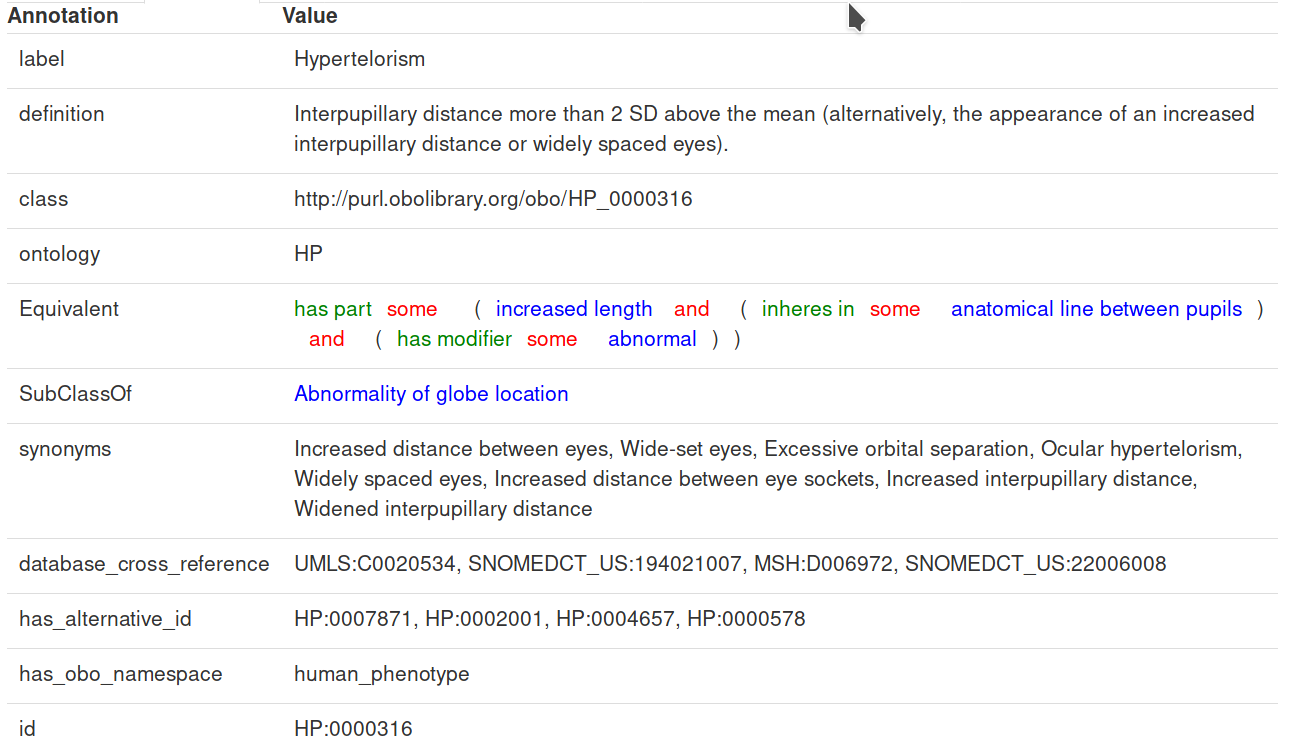
\includegraphics[width=0.8\framewidth]{resources/hyper.png}}
\end{frame}

\begin{frame}{Application Ontologies}
  \begin{itemize}
    \item Rather than categorise very general concepts, some ontologies are
    created around very specific concept areas, by particular methods or for
    particular methods.
    \item Because of their focus on a very specific set of concepts, it allows them to go into a lot of detail, or tailor the conceptualisation around it.
    \item These are known as application ontologies. Sometimes they are built
    into applications or have GUIs for use by clinicians or researchers. 
  \end{itemize}
\end{frame}

\begin{frame}{Application Ontologies: EFO}
  \begin{itemize}
    \item EFO: Experimental Factor Ontology
    \item Developed by EBI to annotate experimental results for their data, and
    to describe the experiments themselves.
    \item Includes classes and relations from many other ontologies, and define
    some of their own specific classes.
    \item Used for the annotation of data in Ensembl, ChEMBL, and the gene
    expression atlas. 
  \end{itemize}
  \centering{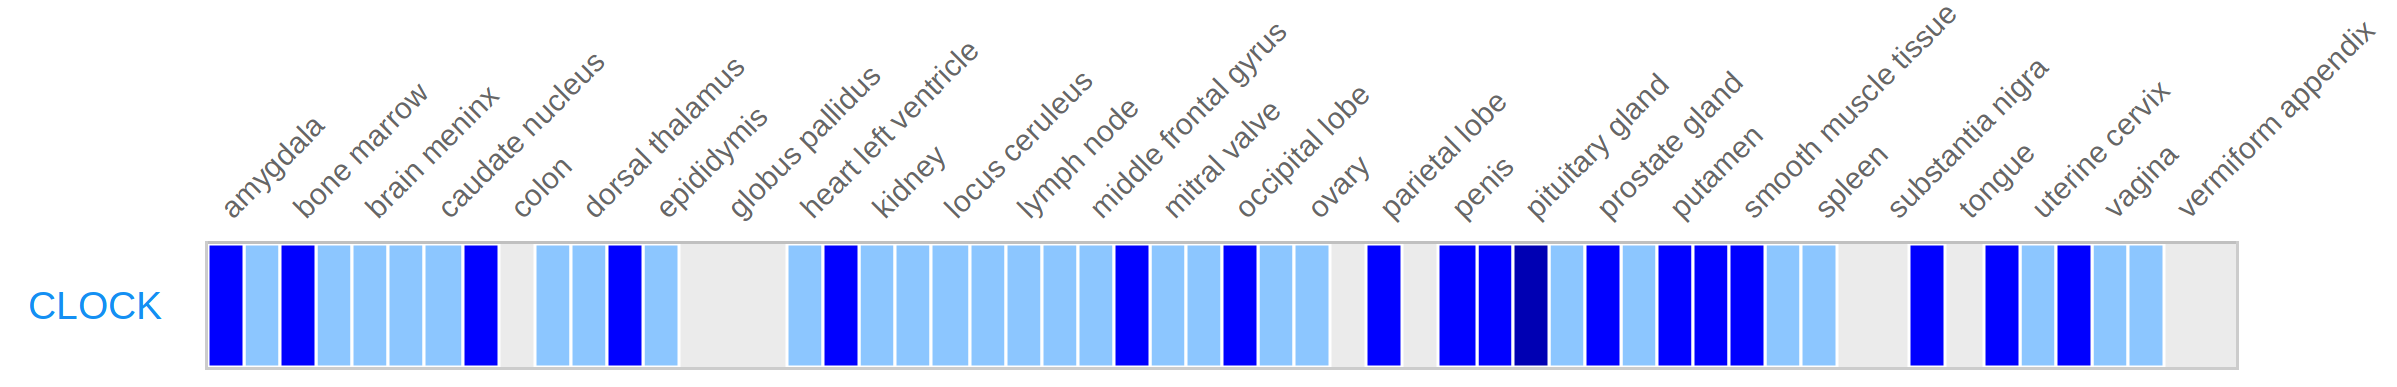
\includegraphics[width=\textwidth]{resources/expression.png}}
\end{frame}

\begin{frame}{Ontology Uses: Annotation}
  \begin{itemize}
    \item The previous was an example of \emph{annotation}.
    \item Annotation is attaching an ontology term to an entity in a database.
    \item By annotating an entity with an ontology term, we are indicating that it is an \emph{instance} of that class.
    \item The annotation link allows us to link up with all the other information connected with the ontology.
    \begin{itemize}
      \item Both in the ontology itself: superclasses, anatomy, side-effects
      \item And in other databases using the ontology annotations: a common schema
    \end{itemize}
  \end{itemize}
\end{frame}

\begin{frame}{Ontology Uses: Uveitis}
  \begin{itemize}
    \item Uveitis is an inflammatory disease of the retina.
    \item The Human Phenotype Ontology already has a definition of uveitis
    (below)
    \item However, what if we want to more deeply characterise phenotypes with
    this disease? And what can we learn from such a characterisation?
  \end{itemize}

  \begin{columns}
    \column{0.5\textwidth}
      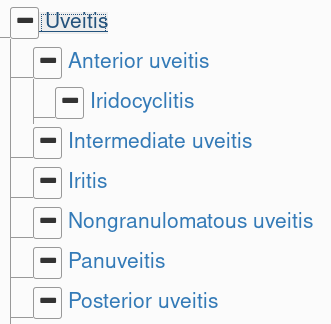
\includegraphics[width=0.5\textwidth]{resources/uveitis.png}
    \column{0.5\textwidth}
      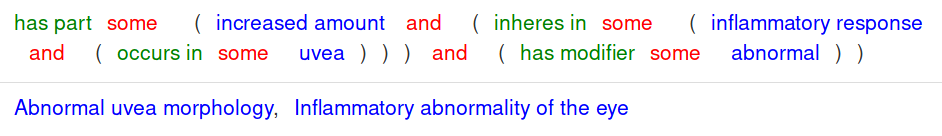
\includegraphics[width=\textwidth]{resources/uv2.png}
  \end{columns}
\end{frame}

\begin{frame}{Ontology Uses: Uveitis}
  \begin{itemize}
    \item An ontology describing the clinical phenotype of Uveitis was built,
    using a clinical document created by Uveitis clinicians
    \item The ontology was then expanded with synonys, using natural language
    processing on a patient discussion forum for the condition
    \item Contains 564 classes describing the phenotype of the disease
  \end{itemize}
\end{frame}

\begin{frame}{Ontology Uses: Uveitis}
  \begin{itemize}
    \item By building the ontology from one patient forum, we were able to
    generalise it to another forum
    \item This also gained us a characterisation of these patients, using which
    we were able to learn about patient experience of the disease
    \item For example, we found with a sentiment analysis that patients were
    less positive if they mentioned anterior uveitis, steroid therapy, or biologic therapy.
  \end{itemize}
\end{frame}

\begin{frame}{Annotation: OMIM}
  \begin{itemize}
    \item Online Mendelian Inheritance in Man
    \item A database of genetic phenotypes, annotated with HPO, and linked to diseases.
    \item We will be using this in the practical later\ldots
  \end{itemize}
\end{frame}

\begin{frame}{OMIM Example}
  \centering{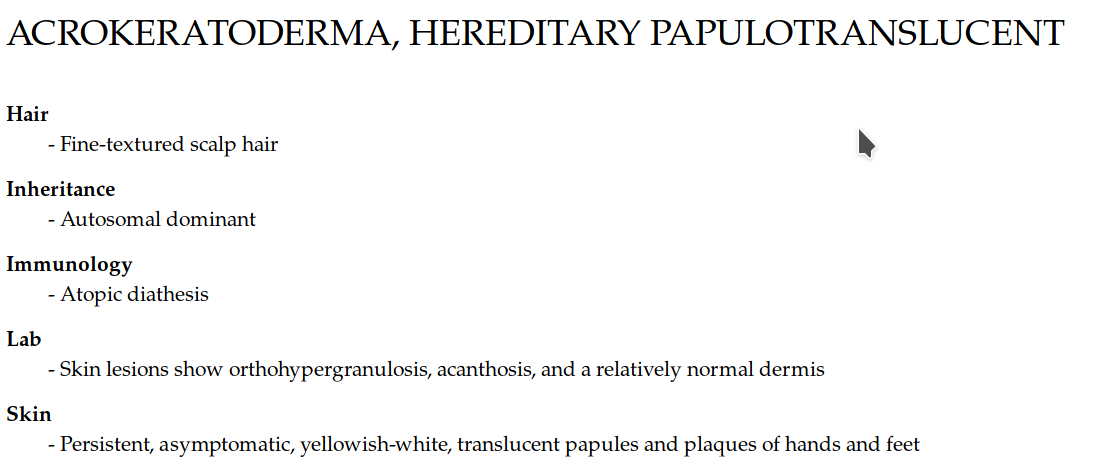
\includegraphics[width=\textwidth]{resources/omim.png}}
\end{frame}

\begin{frame}{Ontology Uses: Semantic Similarity}
  \begin{itemize}
    \item Semantic similarity is a measure of how similar two classes in an
    ontology are, based on the structure of the ontology.
    \item There are many different methods, but most use a form of Information
    Content.
    \item Information Content is a measure of how informative a term is
    \item You can also compare groups of terms, and link these to entities such
    as genes, proteins or diseases.
    \item This is used for protein-protein similarity prediction, disease diagnosis, functional similarity comparison, and more.
  \end{itemize}
\end{frame}

\begin{frame}{Ontology Uses: Vectorisation}
  \begin{itemize}
    \item In Natural Language Processing, word2vec attempts to capture the semantics of a word by recording the words that surround it.
    \item For example, we might get the idea that the symbol `biscuit' is some kind of food because it's commonly used in sentences around verbs like `eat', which is used with other foods.
  \end{itemize}

  \centering{
  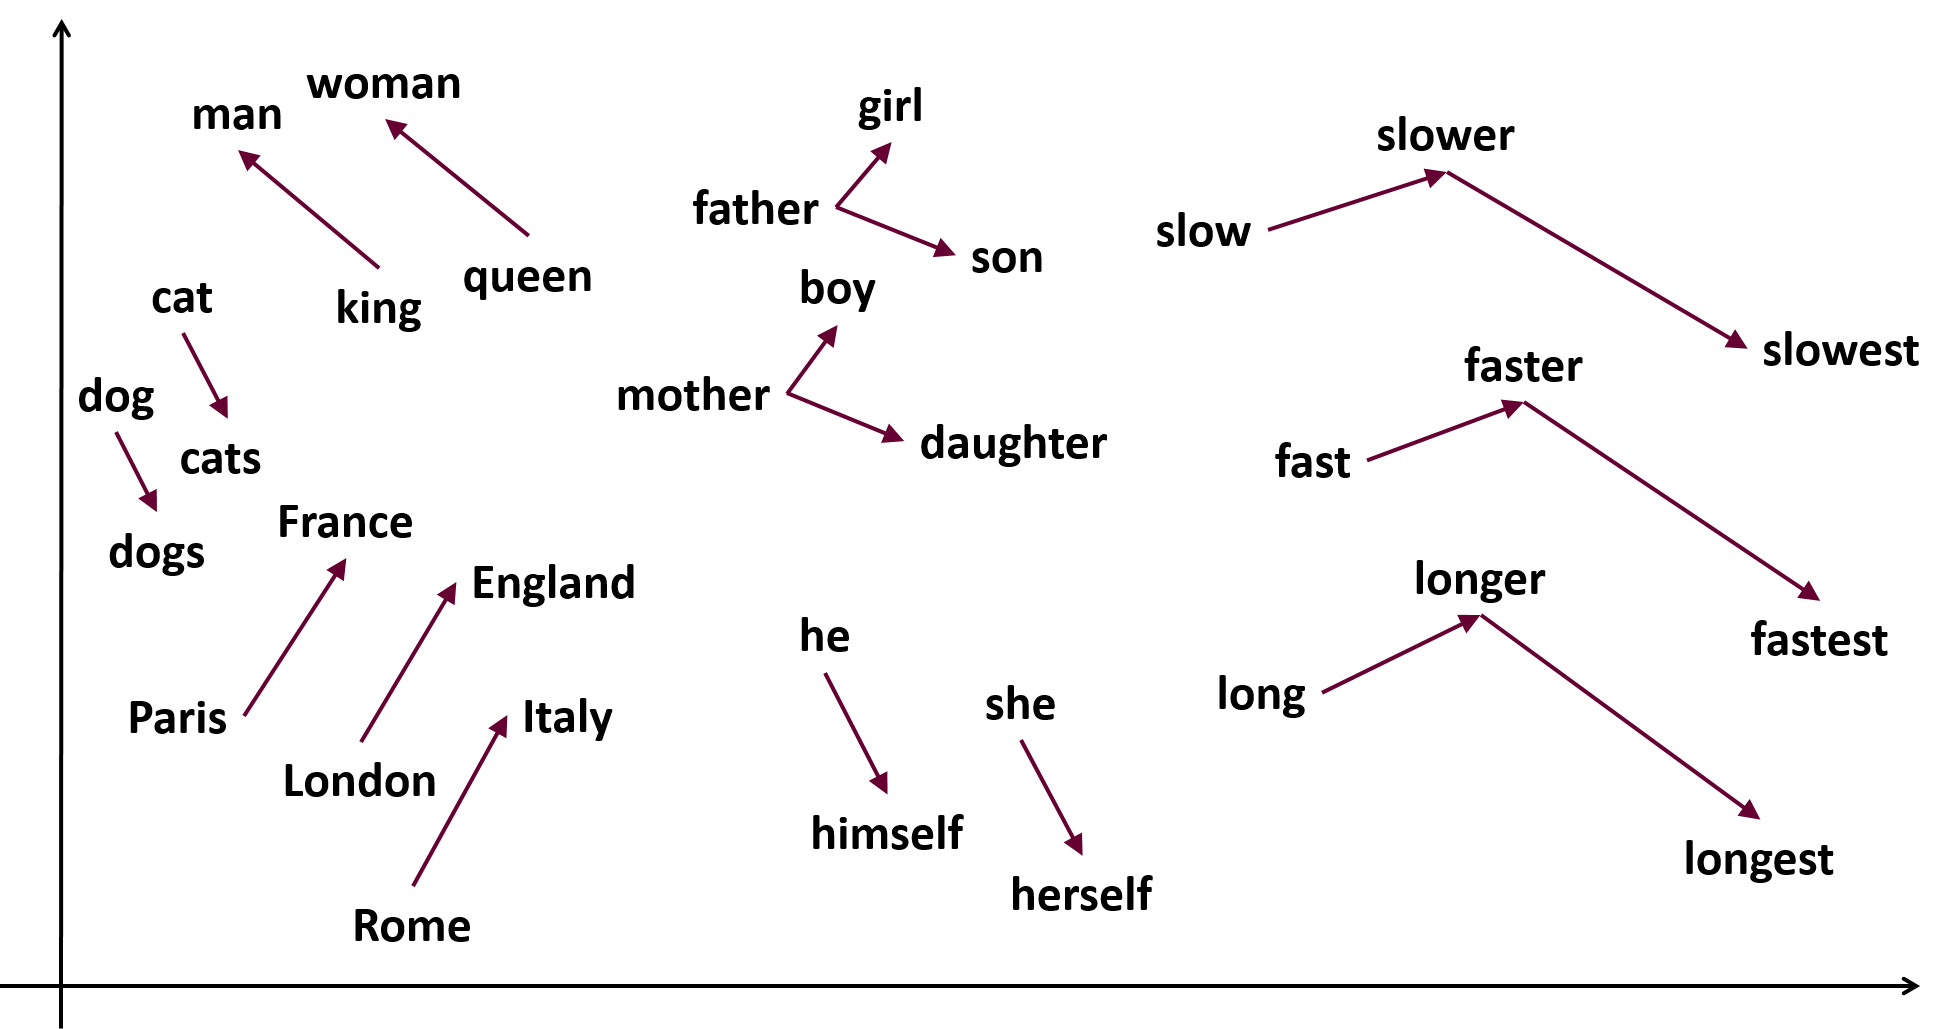
\includegraphics[width=0.65\textwidth]{resources/w2v.png}
  }
\end{frame}

\begin{frame}{Ontology Uses: Vectorisation}

\begin{itemize}
  \item Certain new approaches, such as OPA2Vec, attempt to use `sentences' constructed from ontology axioms to build these similarity vectors
  \item Vectors also have measures of similarity, so we can use them in a similar way to semantic similarity
  \item Vectors can also be used as predictors in machine learning models! This means background information about concepts can be included alongside instance information in predictive models!
\end{itemize}

  has part some (increased amount and (inheres in some (inflammatory response and(occurs in some uvea))) and (has modifier some abnormal))

  \begin{minipage}[t][.2\textheight]{\textwidth}
\tiny{Graphic on previous page taken from https://medium.com/analytics-vidhya/implementing-word2vec-in-tensorflow-44f93cf2665f}
\vfill
\end{minipage}

\end{frame}

\begin{frame}{Ontology Uses: Natural Language Processing}
  \begin{itemize}
    \item We can use ontologies to create vocabulary lists for natural language processing.
    \item When we do this, we also get semantically linked concepts, in the same way that we discussed when we spoke of annotation.
  \end{itemize}
\end{frame}

\begin{frame}{Some Problems in Ontology}
\begin{itemize}
  \item There are more than 550 biomedical ontologies, containing more than
  7,736,665 classes and 80,832,785 axioms.
  \item How can we find what we're looking for?
  \item How can we access and integrate data?
  \item How can we integrate data between ontologies
\end{itemize}
\end{frame}

\begin{frame}{Ontology Repositories}
\begin{itemize}
  \item Ontology repositories allow us to make use of ontology features.
  \item Finding, searching, downloading ontologies. 
  \item Exploring and viewing classes, metadata, links to other databases.
  \item Advanced query functionality and programmatic API (AberOWL has the best one).
  \item Programmatic and interface-based data retrieval from many sources.
  \item Examples: Ontology Lookup Service, AberOWL, Bioportal, OntoQuery
\end{itemize}
\end{frame}

\begin{frame}{Ontology Alignment}
  \begin{itemize}
    \item Ontology alignment finds matches between classes between ontologies. 
    \item For example, there are many different clinical coding systems e.g.
    ICD-10, SNOMED, READCODES.
    \item Another example: Finding class matches between the Human Phenotype
    Ontology, and the Mammalian Phenotype Ontology (mouse). In this case, it can
    help us integrate knowledge from mice and apply it to humans.
    \item There are two main approaches:
      \begin{enumerate}
        \item Lexical: AgreementMakerLite
        \item Semantic: PhenomeNET
        \item Manual: MONARCH
      \end{enumerate}
  \end{itemize}
\end{frame}

\begin{frame}{Some Other Problems in Ontology}
  \begin{itemize}
    \item Lots of people have very different ideas about doing things. There are some ontologies that cover very similar domains, such as the clinical coding ontologies, that are unnecessarily reproducing things and creating an alignment problem!
    \item The people who know how to create and modify ontologies are not the domain experts. This can lead to incorrect knowledge being stored in ontologies.
    \item A lot of knowledge is probabilistic, something that isn't supported by current widely used ontology technology.
  \end{itemize}
\end{frame}

\begin{frame}{Questions}

\end{frame}

\section{Practical}
\begin{frame}[fragile]{Jupyter Notebook on the VM (first time)}
  \tiny
  You will need two(!) separate terminal windows:
  \adjustbox{minipage=1.0\textwidth,scale=0.7}{
    \begin{lstlisting}[language=bash,linewidth=1.2\linewidth]
ssh <username>@172.31.11.61
mkdir module3 # only the first time round
cd module3
git clone https://github.com/athro/msc_bio_module3_practicals.git # only the first time round
module load IPython/6.4.0-foss-2018b-Python-3.6.6
module load scikit-learn/0.20.0-foss-2018b-Python-3.6.6
pip3.6 install bioservices --user } # (you might want to use environments) # only the first time round
jupyter notebook --no-browser 
\end{lstlisting}
}

The output will give you an available port automatically, i.e. the link similar to the following:

\adjustbox{minipage=1.0\textwidth,scale=0.7}{
  \begin{lstlisting}[language=bash,linewidth=1.2\linewidth]
    http://localhost:9014/?token=fb0f0bc5dd12d410bdb7cd1375254e2781d2b544eeea6b5c \end{lstlisting}
}

Take note of this port (in this case 9014) and in {\emph another} terminal window (on your local machine) execute the following command:
\adjustbox{minipage=1.0\textwidth,scale=0.7}{
  \begin{lstlisting}[language=bash,linewidth=1.2\linewidth]
    ssh -N -L <notedport>:172.31.11.61:<notedport> <username>@172.31.11.61  \end{lstlisting}
}

Hopefully you should be able to use the link \url{http://127.0.0.1:<notedport>} on your local browser. 
\end{frame}


\begin{frame}[fragile]{Jupyter Notebook on the VM (afterwards!!)}
  \tiny
  Start with setting up jupyter:
  \adjustbox{minipage=1.0\textwidth,scale=0.7}{
    \begin{lstlisting}[language=bash,linewidth=1.2\linewidth]
ssh <username>@172.31.11.61
cd module3 
module load IPython/6.4.0-foss-2018b-Python-3.6.6
module load scikit-learn/0.20.0-foss-2018b-Python-3.6.6
#git fetch --all # WARNING - this will delete ALL changes you have made
#git reset --hard origin/master # WARNING - this will delete ALL changes you have made
 jupyter notebook --no-browser 
   \end{lstlisting}
 }

 And than start the tunneling in the second terminal window (as about - gain take a not of the port).

\end{frame}

\begin{frame}[fragile]{Jupyter Notebook on own Laptop}
  \begin{itemize}
  \item If possible install  Jupyter Notebook. \url{https://jupyter.readthedocs.io/en/latest/install.html} for Python 3.7
  \item Within your terminal install bioservice\\
    \adjustbox{minipage=1.0\textwidth,scale=0.75}{
      \begin{lstlisting}[language=bash,linewidth=1.2\linewidth]
        pip install --user bioservices # please check if you have to use pip3 or pip3.6
      \end{lstlisting}
   }
  \item No pip? Install: \url{ https://pip.pypa.io/en/latest/installing/}
  \item Create and goto the folder {\verb module3 } and clone the practical repository (see slide before)
  \item Start the notebook
    
  \adjustbox{minipage=1.0\textwidth,scale=0.75}{
    \begin{lstlisting}[language=bash,linewidth=1.2\linewidth]
      mkdir module3 
      cd module3
      git clone https://github.com/athro/msc_bio_module3_practicals.git
      jupyter notebook --no-browser --port=9000
    \end{lstlisting}
  }
    
  \end{itemize}
\end{frame}


\begin{frame}[fragile]{Clean pull - ignoring all local changes}

  To get a clean pull from a git repository, i.e. one that overides any changes on your local filestore:
  
  \adjustbox{minipage=1.0\textwidth,scale=0.75}{
  \begin{lstlisting}[language=bash,linewidth=1.2\linewidth]
    git fetch --all
    git reset --hard origin/master
  \end{lstlisting}
  }
\end{frame}


\end{document}
